\documentclass[11pt]{article}
\usepackage{array, xcolor}
\usepackage[margin=1.5cm]{geometry}
\usepackage{hyperref}

\usepackage{graphicx,mwe}
\usepackage{array}
\usepackage{graphicx}
\usepackage{wrapfig}

\usepackage{enumitem}

\usepackage{fontspec}
\setmainfont{Helvetica}
\setsansfont{DejaVu Sans}
\setmonofont{DejaVu Sans Mono}
\usepackage{fontsize}
\changefontsize[13]{12}
 
 \usepackage[none]{hyphenat}
  
\title{\bfseries\Huge Oleg Shpynov}
\author{\textbf{oleg.shpynov@gmail.com}}
\date{}
 
\definecolor{lightgray}{gray}{0.8}
\newcolumntype{L}{>{\raggedleft}p{0.16\textwidth}}
\newcolumntype{R}{p{0.8\textwidth}}
\newcommand\VRule{\color{lightgray}\vrule width 0.5pt}
 
%%% Begin Document
\begin{document}
\maketitle 

\begin{wrapfigure}{r}{0.4\textwidth}
    \vspace*{-4cm} % moving actual picture up
	\hfill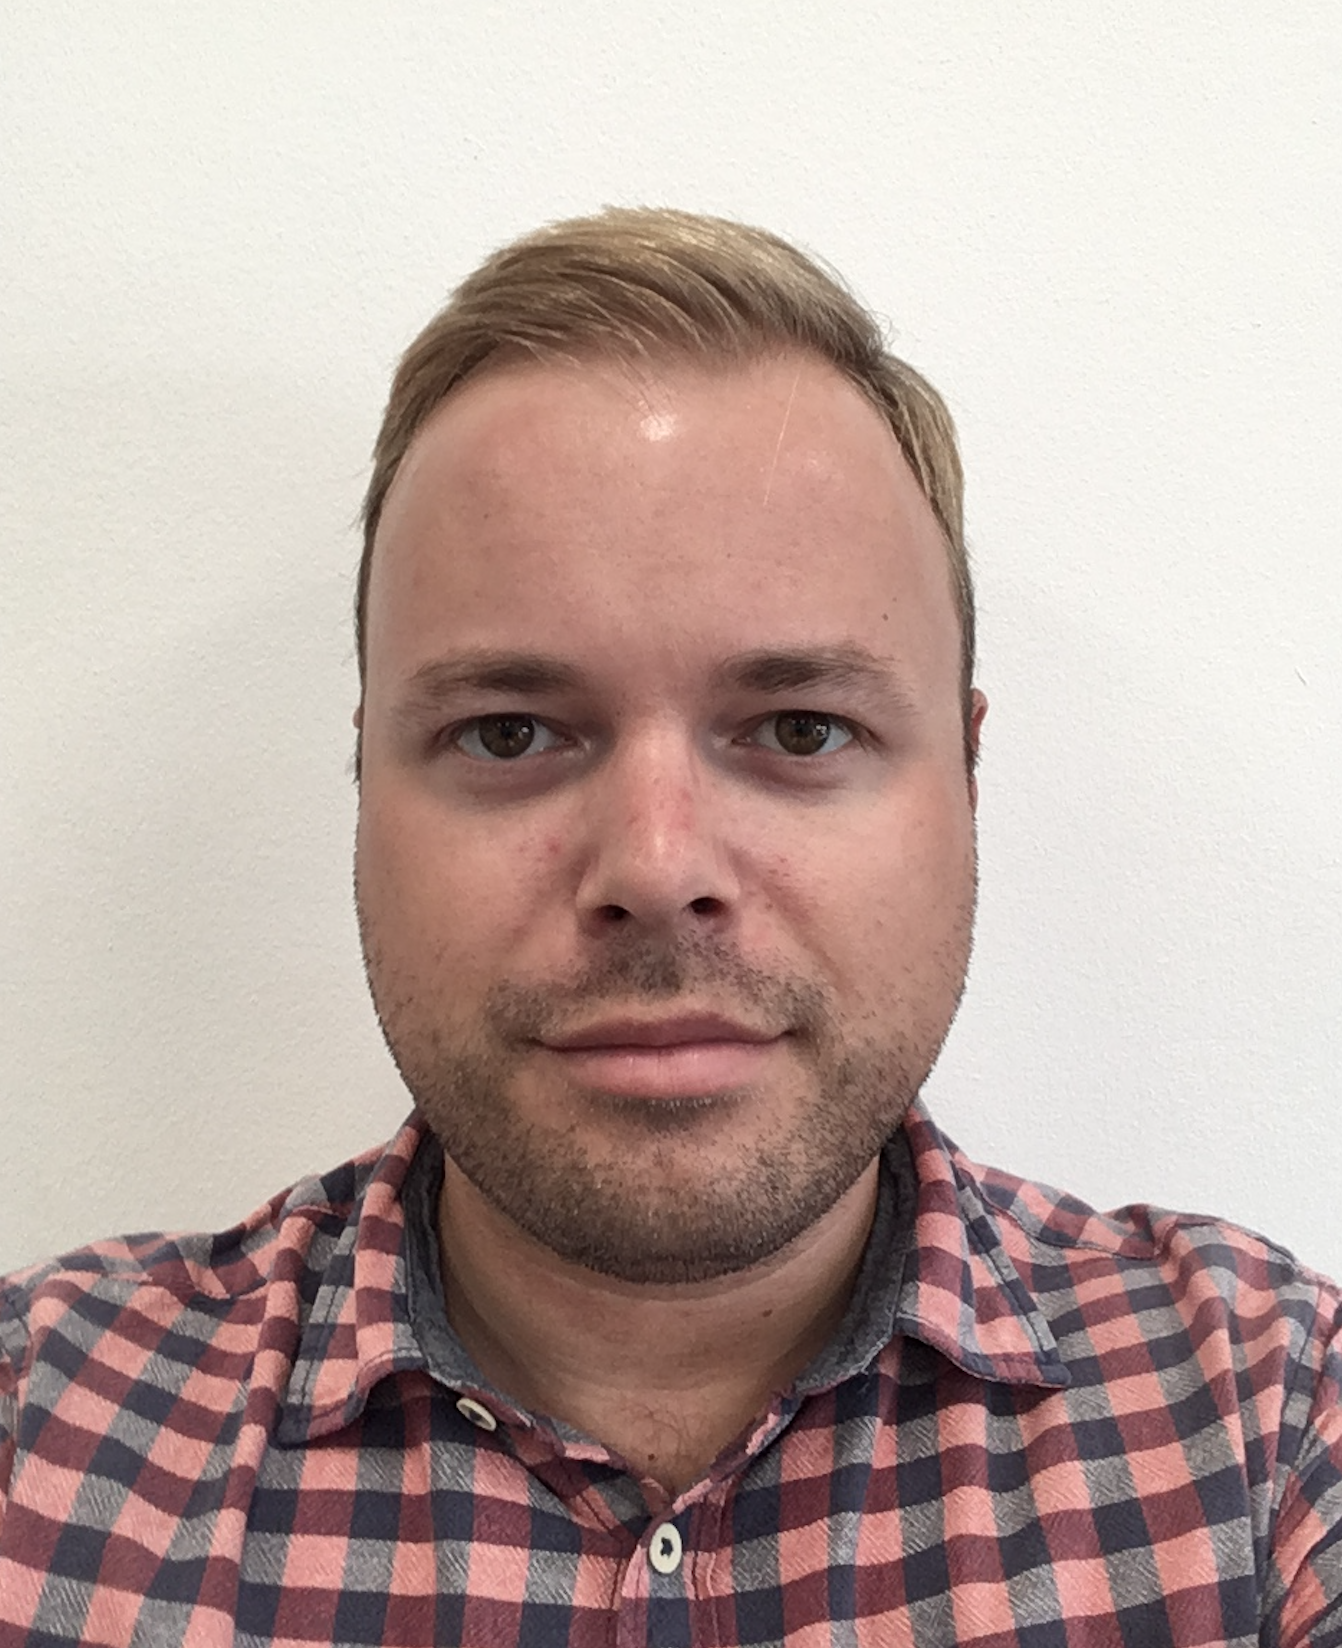
\includegraphics[width=0.20\textwidth]{me2020.png}
    \vspace*{-4cm} % avoid real text wrapping
\end{wrapfigure}



%%% Personal details
\hspace*{-0.6cm}\begin{minipage}[ht]{0.4\textwidth}
80999 Waltenbergerstr. 11\\
Munich, Germany
\end{minipage}
\begin{minipage}[ht]{0.4\textwidth}
April 7th, 1986\\
+ 49 177 6904790
\end{minipage}
\vspace{10pt}

%%% About me short
\section*{Summary}
Bioinformatics group leader with software development expertise at JetBrains Research.
Graduated cum laude from Saint-Petersburg State University in 2008 and received Master degree in Computer Science.
Now working on computational algorithms and methods for epigenetic data analysis in the field of human aging
with a specific focus on ChIP-seq and ATAC-seq methods under the supervision of Dr. Maxim Artyomov, Washington University of St.Louis.

%%% Research experience
\section*{Research Experience}
\begin{tabular}{L!{\VRule}R}

2016 -- today & \textbf{Bioinformatics Group Leader}\\
& \textit{JetBrains Research, Munich, Germany}\\[5pt]
& \href{http://research.jetbrains.org/groups/biolabs}{BioLabs} group is developing novel algorithms and methods for experimental data analysis, building scalable computational pipelines and tools, and working in collaboration with biologists on various ageing studies.\\
& \setlist{nolistsep}
\begin{itemize}[noitemsep]
	\item Data analysis of various biological experimental datasets
   \item Created novel peak calling solution for ChIP-seq and ATAC-seq data analysis - semi-supervised peak caller
  \href{https://github.com/jetBrains-Research/span}{SPAN} and \href{https://github.com/jetBrains-Research/jbr}{JBR} Genome Browser
  \item Developed \href{https://github.com/jetBrains-Research/pubtrends}{PubTrends} - exploratory tool
  for scientific publications providing faster trends analysis and breakthrough papers discovery
  \item Participated in development of \href{https://plugins.jetbrains.com/plugin/11947-snakecharm}{SnakeCharm} -
smart editor plugin of \href{https://snakemake.readthedocs.io/en/stable/}{Snakemake} workflow description language for  \href{https://www.jetbrains.com/pycharm/features/}{PyCharm} IDE
\end{itemize}\\

2017 -- 2019 & \textbf{Visiting Research Scientist}\\
& \textit{Department of Pathology and Immunology, Washington University,} \\
& \textit{St. Louis, MO, USA}\\[5pt]
& Working on applied machine learning approaches and methods for epigenetic data analysis under supervision of Dr. Maxim Artyomov.\\
& \setlist{nolistsep}
\begin{itemize}[noitemsep]
	\item Developed scalable, reproducible computational pipelines for ChIP-seq processing
	\item Created pipelines for single cell  ATAC-seq analysis
	\item Analyzed of Ultra-Low Input ChIP-seq datasets and single cell ATAC-seq datasets
\end{itemize}\\

\end{tabular}

%%% Teaching experience
\section*{Teaching Experience}
\begin{tabular}{L!{\VRule}R}
2022 & \textbf{Lecturer}\\
& \textit{Constructor Univeristy, Bremen, Germany}\\
& \setlist{nolistsep}
\begin{itemize}[noitemsep]
	\item Course "Algorithmic Bioinformatics" for Bachelor students. The course covers various bioinformatic algorithms actively used in computational and systems biology. Theoretical background is complemented by solving practical problems.
\end{itemize}\\
2019 - 2022 & \textbf{Lecturer}\\
& \textit{University ITMO, Saint-Petersburg, Russia}\\
& \setlist{nolistsep}
\begin{itemize}[noitemsep]
	\item Course "Computational Analysis of Epigenetic Data" for Master's Students in the "Bioinformatics and Systems Biology" \href{https://en.itmo.ru/en/viewjep/2/54/Bioinformatics_and_Systems_Biology.html }{program}. The course covers foundations of epigenetic regulation of transcription and computational approaches of ChIP-seq and WGBS data analysis and integration.
\end{itemize}\\
2018 -- 2020 & \textbf{Speaker}\\
& \textit{Systems Biology Workshop, Saint-Petersburg, Russia}\\
& \setlist{nolistsep}
\begin{itemize}[noitemsep]
	\item{System level data ranging from gene expression, RNA-, ChIP-, and exome-sequencing up to high-throughput metabolomics and network-based data integration. Joint workshop with Washington University in St.Louis, Dr. Maxim Artyomov.}
\end{itemize}\\
2014 -- 2022 & \textbf{Students Mentor}\\
& \textit{Bioinformatics Institute, Saint-Petersburg, Russia}\\
& \textit{Computer Science Center, Saint-Petersburg, Russia}\\
& \textit{Higher School of Economics, Saint-Petersburg, Russia}\\
& \setlist{nolistsep}
\begin{itemize}[noitemsep]
  \item Supervisor of two successful Masters dissertations
  \item Mentorship of various students projects
  \item Seminars
\end{itemize}\\
\end{tabular}


%%% Professional experience
\section*{Professional Experience}
\begin{tabular}{L!{\VRule}R}
2006 -- 2013 & \textbf{Senior Software Developer}\\
& \textit{JetBrains, Saint-Petersburg, Russia}\\[5pt]
& Main focus was on the analysis of source code in programming languages, starting from lexical analysis to advanced type system development and source code semantic verifications.\\
& \setlist{nolistsep}
\begin{itemize}[noitemsep]
	\item Developed JetBrains products: flagship tool \href{https://jetbrains.com/idea}{IntellIJ IDEA}, \href{https://jetbrains.com/pycharm}{PyCharm}
	\item Maintained and developed \href{https://plugins.jetbrains.com/plugin/164?pr=idea}{IdeaVIM} plugin (vim emulation plugin, 7+mln downloads)
	\item Created \href{http://jetbrains.com/ruby}{RubyMine} Integrated Development Environment for Ruby programming language and Ruby On Rails technology
\end{itemize}
\end{tabular}

%%% Education
\section*{Education}
\begin{tabular}{L!{\VRule}R}
2016 & Systems Biology Workshop by Bioinformatics Institute, ITMO University and Washington University in St.Louis, Saint-Petersburg, Russia \\
& \\
2011 -- 2012 & Saint-Petersburg Academic University — Nanotechnology Research and Education Centre of the Russian Academy of Sciences, Russia\\
& Introduction to bioinformatics, molecular biology, statistics. \\
& \\
2003 -- 2008 & Masters in Computer Science, 4.9 of 5. Saint-Petersburg State University, Russia \\
& Faculty of Mathematics and Mechanics, Department of System Programming \\
\end{tabular}
 
\section*{Publications}
\begin{tabular}{L!{\VRule}R}
2021 & \textbf{Oleg Shpynov}, Aleksei Dievskii, Roman Chernyatchik, Petr Tsurinov, Maxim N Artyomov, "Semi-supervised peak calling with SPAN and JBR genome browser"; Bioinformatics 37 (22), 4235-4237\\
& website \href{https://artyomovlab.wustl.edu/aging/tools.html/}{https://artyomovlab.wustl.edu/aging/tools.html}\\
& \\
2020 & Irina Shchukina, Juhi Bagaitkar, \textbf{Oleg Shpynov*}, Ekaterina Loginicheva, Sofia Porter, Denis A Mogilenko, Erica Wolin, Patrick Collins, German Demidov, Mykyta Artomov, Konstantin Zaitsev, Sviatoslav Sidorov, Christina Camell, Monika Bambouskova, Laura Arthur, Amanda Swain, Alexandra Panteleeva, Aleksei Dievskii, Evgeny Kurbatsky, Petr Tsurinov, Roman Chernyatchik, Vishwa Deep Dixit, Marko Jovanovic, Sheila A Stewart, Mark J Daly, Sergey Dmitriev, Eugene M Oltz, Maxim N Artyomov, "Enhanced epigenetic profiling of classical human monocytes reveals a specific signature of healthy aging in the DNA methylome"; Nature aging 1 (1), 124-141 \\
& website \href{https://artyomovlab.wustl.edu/aging/}{https://artyomovlab.wustl.edu/aging/}\\
& \\
2020 & Denis A. Mogilenko, \textbf{Oleg Shpynov}, Prabhakar Sairam Andhey, Laura Arthur, Amanda Swain, Ekaterina Esaulova, Simone Brioschi, Irina Shchukina, Martina Kerndl, Monika Bambouskova, Zhangting Yao, Anwesha Laha, Konstantin Zaitsev, Samantha Burdess, Susan Gillfilan, Sheila A. Stewart, Marco Colonna, Maxim N. Artyomov,, "Comprehensive profiling of an aging immune system reveals clonal GZMK+ CD8+ T cells as conserved hallmark of inflammaging"; Immunity, Immunity 54 (1), 99-115. e12 \\
&  website \href{https://artyomovlab.wustl.edu/immune-aging/}{https://artyomovlab.wustl.edu/immune-aging/}\\
& \\
2020 & Anna Nikiforovskaya, Nikolai Kapralov, Anna Vlasova, \textbf{Oleg Shpynov}, Aleksei Shpilman,  "Automatic generation of reviews of scientific papers"; 2020 19th IEEE International Conference on Machine Learning and Applications \\
& \\
2018 & Jeremy P. Huynh, Chih-Chung Lin, Jacqueline M. Kimmey, Nicholas N. Jarjour, Elizabeth A. Schwarzkopf, Tara R. Bradstreet, Irina Shchukina, \textbf{Oleg Shpynov}, Casey T. Weaver, Reshma Taneja, Maxim N. Artyomov, Brian T. Edelson, Christina L. Stallings, "Bhlhe40 is an essential repressor of IL-10 during Mycobacterium tuberculosis infection"; Journal of Experimental Medicine 2 July 2018; 215 (7): 1823–1838\\
& \\
& \\
& \textit{* - first co-author}
\end{tabular}

\section*{Languages}
\begin{tabular}{L!{\VRule}R}
Russian & Native\\
English & Fluent\\
Germany & Elementary\\
\end{tabular}

\section*{Courses}
\begin{tabular}{L R}
& Deep learning nanodegree at Udacity, certificate number: 9GSNRHUA  \\
& Machine learning, deep learning, models deployment
\end{tabular}

\section*{Honors and Awards}
\begin{tabular}{L R}
& ACM ICPC regional contests paricipant in university team \\
&  Winner of Saint-Petersburg State school contests on Mathematics, Physics, and Programming
\end{tabular}

\section*{Interests}
\begin{tabular}{L R}
	& Bioinformatics, machine learning, software development.\\
	& Spending time with family, traveling, snowboarding, photography. \\
\end{tabular}
 
\end{document}